% One-slide talk (O-slide). Compile:  cd slides && xelatex oneslide.tex
% The figure is produced by code/plots.py -> figures/main_figure.pdf
\documentclass[aspectratio=169,10pt]{beamer}
\usepackage{fontspec}
\usepackage{polyglossia}
\setdefaultlanguage{russian}
\setotherlanguage{english}
\setmainfont{DejaVu Sans}
\setsansfont{DejaVu Sans}
\setmonofont{DejaVu Sans Mono}
\newfontfamily\condensed{DejaVu Sans Condensed}
\usepackage{unicode-math}
\setmathfont{Latin Modern Math}
\usepackage{graphicx}

\definecolor{ink}{HTML}{0B0B0B}
\definecolor{ink2}{HTML}{52514E}
\definecolor{accent}{HTML}{1C5CAB}
\setbeamertemplate{navigation symbols}{}
\setbeamercolor{normal text}{fg=ink}
\setbeamercolor{frametitle}{fg=accent}
\setbeamerfont{frametitle}{size=\large,series=\bfseries}
\setbeamersize{text margin left=5mm,text margin right=5mm}
\setbeamertemplate{frametitle}{\vspace*{1.5mm}\insertframetitle\par\vspace{0.5mm}
  {\normalfont\fontsize{8}{9.5}\selectfont\color{ink2}\insertframesubtitle\par}}
\setbeamertemplate{footline}{\hbox to \paperwidth{\hspace*{5mm}\fontsize{5.5}{6.5}\selectfont\color{ink2}%
  ВМК МГУ\enspace·\enspace «Моя первая научная статья», 2026%
  \hfill вычисления: \texttt{code/main.py}\enspace·\enspace рисунок: \texttt{code/plots.py}\hspace*{5mm}}\vspace*{2mm}}

\newcommand{\head}[1]{{\fontsize{7.8}{9}\selectfont\color{accent}\bfseries #1}\par\vspace{0.4mm}}
\newcommand{\colfont}{\condensed\fontsize{7}{8.2}\selectfont}
\newcommand{\thesis}[1]{\par\vspace{0.9mm}{\bfseries\color{accent}#1}\ }

\begin{document}
\begin{frame}[t]
\frametitle{Признаки слова заменяют часть опроса носителей}
\framesubtitle{Иерархическая модель Брэдли–Терри для ранжирования татарских замен русских заимствований}

\vspace{-1.5mm}
\begin{columns}[T,onlytextwidth]
\begin{column}{0.29\textwidth}\colfont\raggedright
\vspace{1mm}
\head{Что и зачем}
\thesis{Задача.} Упорядочить татарские замены заимствования по мнению носителей.
\thesis{Проблема.} Опрос носителей дорог, у новых слов нет истории оценок.
\thesis{Идея.} Признаки слова — априорная оценка, сравнения её уточняют.
\thesis{Вопрос.} Сколько сравнений экономят признаки и при каком $\rho$?
\thesis{Зачем.} Спланировать опрос; метод общий для попарных оценок.
\end{column}
\begin{column}{0.69\textwidth}
\centering
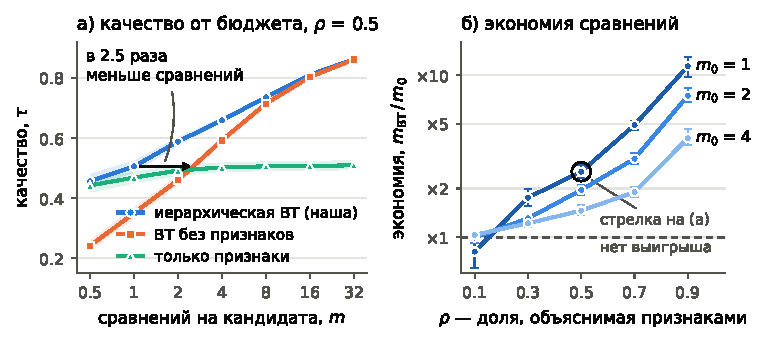
\includegraphics[width=0.92\linewidth]{../figures/main_figure_slide.pdf}
\end{column}
\end{columns}

\vspace{0.8mm}
\begin{columns}[T,onlytextwidth]
\begin{column}{0.36\textwidth}\colfont\raggedright
\head{Модель}
\hspace*{2mm}$P(w_i \succ w_j)=\sigma(u_i-u_j),\;\; u_i=\theta^{\top}\mathbf{x}_i+\eta_i$;\\[0.4mm]
$\mathbf{x}_i$ — признаки слова (план: «татарскость» по символьной LM, сингармонизм, длина\,…; в синтетике — случайные), $\eta_i$ — то, что признаки не объясняют.
\end{column}
\begin{column}{0.29\textwidth}\colfont\raggedright
\head{Обозначения}
$m$ — сравнений на кандидата;\\
$\tau$ — Кендалл с истинным порядком;\\
$\rho$ — доля разброса предпочтений, объяснимая признаками;\\
$m_{\mathrm{BT}}/m_0$ — во сколько раз длиннее опрос без признаков.
\end{column}
\begin{column}{0.31\textwidth}\colfont\raggedright
\head{Результат}
При $\rho=0.5$ одного сравнения на кандидата хватает там, где BT без признаков нужно~$2.5$; при $\rho=0.9$ — в~$11$ раз меньше. Бесполезные признаки ($\rho=0.1$) не помогают, а при $m=1$ слегка мешают.\\[0.5mm]
{\color{ink2}Синтетика: 40 заимствований $\times$ 8 кандидатов, 20 запусков, 95\%-е ДИ.}
\end{column}
\end{columns}
\end{frame}
\end{document}
